\documentclass[titlepage,a4paper]{article}

\usepackage{a4wide}
\usepackage[colorlinks=true,linkcolor=black,urlcolor=blue,bookmarksopen=true]{hyperref}
\usepackage{bookmark}
\usepackage{fancyhdr}
\usepackage[spanish]{babel}
\usepackage[utf8]{inputenc}
\usepackage[T1]{fontenc}
\usepackage{graphicx}
\usepackage{float}

\pagestyle{fancy} % Encabezado y pie de página
\fancyhf{}
\fancyhead[L]{TP2S }
\fancyhead[R]{Algoritmos y Programación III - FIUBA}
\renewcommand{\headrulewidth}{0.4pt}
\fancyfoot[C]{\thepage}
\renewcommand{\footrulewidth}{0.4pt}

\begin{document}
\begin{titlepage} % Carátula
	\hfill
\includegraphics[width=6cm]{logofiuba.jpg}
    \centering
    \vfill
    \Huge \textbf{Trabajo Práctico 2 — Java}
    \vskip2cm
    \Large [7507/9502] Algoritmos y Programación III\\
    Curso 1 \\ % Curso 1 para el de la tarde y 2 para el de la noche
    Segundo cuatrimestre de 2019 
    \vfill
    \begin{tabular}{ | l | l | l | } % Datos del alumno
     
                
       \hline
      Alumno: & PRATTO, Federico \\ \hline
      Número de padrón: & 96223 \\ \hline
      Email: & fpratto@fi.uba.ar \\ \hline
     
      \hline
      Alumno: & BUCETA , M. Belén \\ \hline
      Número de padrón: & 102121 \\ \hline
      Email: & bucetabmb@gmail.com \\ \hline

       
      Alumno: & DI COMO, Juan Pablo \\ \hline
      Número de padrón: & 102889 \\ \hline
      Email: & jdicomo@fi.uba.ar \\ \hline  
      

  	\end{tabular}
    \vfill
    \vfill
\end{titlepage}

\tableofcontents % Índice general
\newpage

\section{Introducción}\label{sec:intro}
El presente informe reune la documentación de la solución del segundo trabajo práctico de la materia Algoritmos y Programación III que consiste en desarrollar una aplicación de un videojuego 'AlgoChess' en Java con un diseño del modelo orientado a objetos y trabajando con las técnicas de TDD e Integración Contínua.


\section{Supuestos}\label{sec:supuestos}
% Deberá contener explicaciones de cada uno de los supuestos que el alumno haya tenido que adoptar a partir de situaciones que no estén contempladas en la especificación.

-Al comienzo del juego, cada jugador puede colocar sus unidades solo en sus territorios. Luego de dar por comenzado el juego, es decir, una vez que cada jugador coloco sus unidades, sí tiene la posibilidad de mover sus fichas hacia territorio enemigo. 

-Una unidad que se encuentre en un casillero enemigo puede ser curado por un curandero de su mismo bando, sin aplicarle ninguna sanción por encontrarse en sector enemigo. 


-Una catapulta atacante, puede atacar sólo a enemigos pero puede en esa acción dañar a enemigos y aliados. Ya que durante el ataque pueden encontrarse aliados contiguos que sufren daños. 

-Un curandero puede ser atacado. 

-Ninguna unidad puede usar su habilidad consigo misma. 

-Ninguna unidad puede atacar a una otra aliada.

-Batallón: 

Un batallón es una situación que ocurrirá en caso de que ocurra durante el moviento de un soldado. Es decir, no está en responsabilidad de un jugador definir si quiere usar o no un batallón. En caso de formarse uno, el movimiento se realizará como batallón. 

Un batallón solo se conforma por soldados aliados y ninguna otra unidad.

Un batallón tiene tres integrantes. 

Al seleccionar un Soldado para moverlo, el Tablero se fija si tiene dos soldados que sean vecinos inmediatos, es decir, si se ubican a un casillero de distancia en alguna dirección (formando una recta entre los tres).

Una importante observación es resaltar que el hecho de que ocurra un batallón no implica que éste vaya a moverse. Para ello debe darse que puedan hacerlo en las direcciones correspondientes a cada uno de sus respectivos desplazamientos. 


Otra observación: solo se permite un batallón por turno. Esto significa que aunque en el turno se halle la posibilidad de formar más de un batallón en distintos sentidos, el batallón que se concretará será aquel que primero se encuentre y ningún otro más se formará en dicho turno. 


- Vista

Está permitido que un jugador decida no comprar unidades al comenzar el juego. En dicho caso, el juego dará comienzo y al finalar el primer turno; el juego se dará por finalizado. 



\begin{figure}[H]
\centering
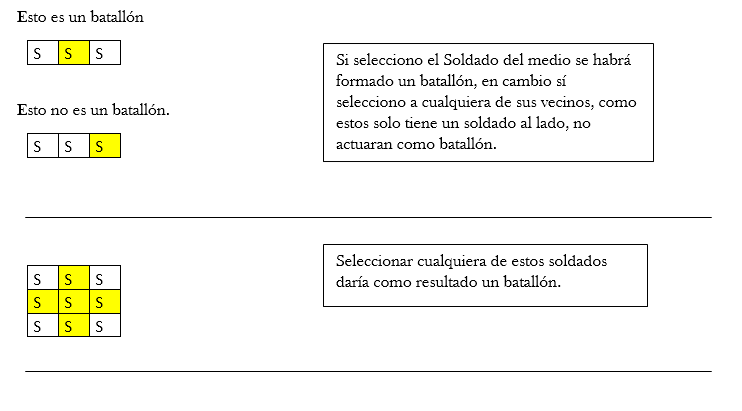
\includegraphics[width=0.8\textwidth]{FormacionBatallon.png}
\caption{\label{fig:seq01}. Formación de un Batallón}
\end{figure}

Por otro lado, el sentido en el que se realiza la búsqueda de un batallón se determinó en el siguiente orden. Primero, en sentido vertical,  luego horinzontal, siguiendo con  creciente en dirección noreste y finalmente creciente en diagonal noroeste. Una vez hallado un batallón se detiene la búsqueda. 
Para mayor comprensión se adjunta un gráfico con cada caso. 

\begin{figure}[H]
\centering
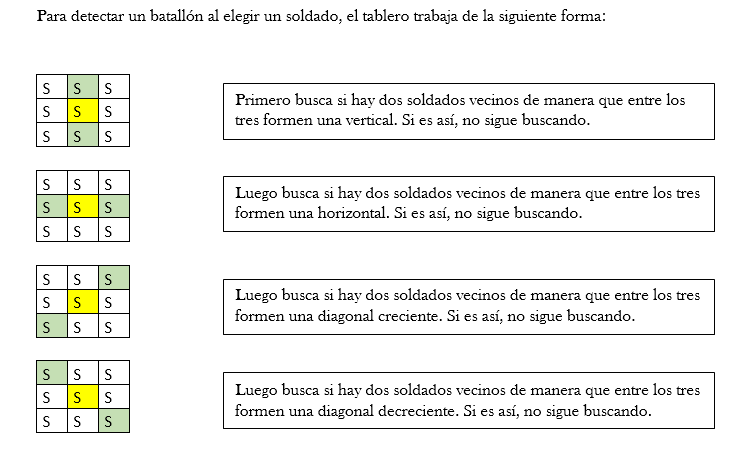
\includegraphics[width=0.8\textwidth]{DeteccionBatallon.png}
\caption{\label{fig:seq01}. Detección de un Batallón}
\end{figure}


\begin{itemize}
\item Movimiento de un Batallón:
\end{itemize}
Si se ha encontrado un batallon, el tablero intentará mover las tres unidades 		en la direccion solicitada, si no logra mover ninguna pieza debido a que todas están 	  bloqueadas lanzará un error. 

Considere que al mover un batallón, si la pieza que se elige mover se encuentra entre medio de sus soldados aliados, el movimiento de todo el batallón será exitosa en cuanto no se encuentre bloqueado por algún obstáculo (salirse del tablero, encontrarse con una pieza que ocupe el casillero donde se buscaba mover el soldado que se eligió mover). Los soldados que se encuentran a sus dos lados, compañeros de batallón no suponen un obstáculo. 

Por otro lado, en caso de elegirse mover alguno de los soldados de los extremos del batallón debe tenerse en cuenta que:

-Si el soldado del extremo elegido debe moverse hacia la posición ocupada por su soldado aliado contiguo (integrante del batallón) entonces, el movimiento no será exitosa pues el habrá una excepción de casillero ocupado. En ese caso, el compañero de batallón si resulta ser un obstáculo.

-Si el soldado del extremo elegido para moverse debe moverse hacia una posición que se encuentra desocupada, es decir, su soldado aliado compañero de batallón no se encuentra allí, entonces el movimiento del batallón será exitoso. 

Nota: se dice que un soldado es elegido para moverse cuando el jugador mueve una pieza específica. 




\section{Modelo de dominio}\label{sec:modelo}
% Explicación concisa del diseño general del trabajo.


En primer lugar, pasaremos a explicar cuáles son los objetos más relevantes que  intervienen en el diseño del modelo, con el objetivo de clarificar la lógica que utilizamos para resolver el trabajo.
Cada objeto explicado a continuación fue creado con el fin de resolver contextos pequeños y específicos de manera ordenada y simple, y que sean relevantes a él. 

Jugador: Es un participante del juego. Un jugador dispone de puntos para obtener unidades y también posee un bando, del cual sus unidades (o más claramente entendidas como sus 'fichas' para jugar) son miembros del mismo. 

Unidad: Cada personaje del juego: Un soldado, jinete, catapulta y curandero constituye una unidad. En términos de implementación, la unidad es una superclase de la cual dichos personajes heredan como subclases. La unidad tiene asociado un bando específico que se corresponde con el mismo del jugador que la posee. También está asociada a una habilidad específica, que puede usarse siempre que se cumplan las condiciones establecidas para esa determinada habilidad por las reglas del juego. Y también se asocia a un casillero donde se encuentra alojada dicha unidad. 

Habilidad: Puede definirse como una acción que puede hacer una unidad, existen muchos tipos de habilidades dentro del juego. En especial, dentro del juego se definieron como habilidades, AtaqueCerca, AtaqueMedio, AtaqueEnArea, Curación, todos ellos constituyen subclases de la clase madre Habilidad. A su vez, una habilidad tiene un poder, es la capacidad de daño que puede generarle una unidad a una unidad enemiga. Y también está asociada a un Alcance. 

Alcance: Esta clase tiene un propósito de medir distancias. Posee atributos de distancia Máxima y mínima. 

Casillero: Es el lugar donde es ubicada una unidad dentro del juego.  Un casillero tiene un Estado que puede ser libre o ocupado. También está asignado a un determinado bando pero éste no necesariamente corresponde al mismo del jugador. A su vez, un casillero conoce a sus casilleros vecinos. Se entiende por vecino a todo casillero adyacente (en cualquier dirección) al casillero seleccionado. 


\section{Diagramas de clase}\label{sec:diagramasdeclase}
% Uno o varios diagramas de clases mostrando las relaciones estáticas entre las clases.  Puede agregarse todo el texto necesario para aclarar y explicar su diseño. Recuerden que la idea de todo el documento es que quede documentado y entendible cómo está implementada la solución.



\begin{figure}[H]
\centering
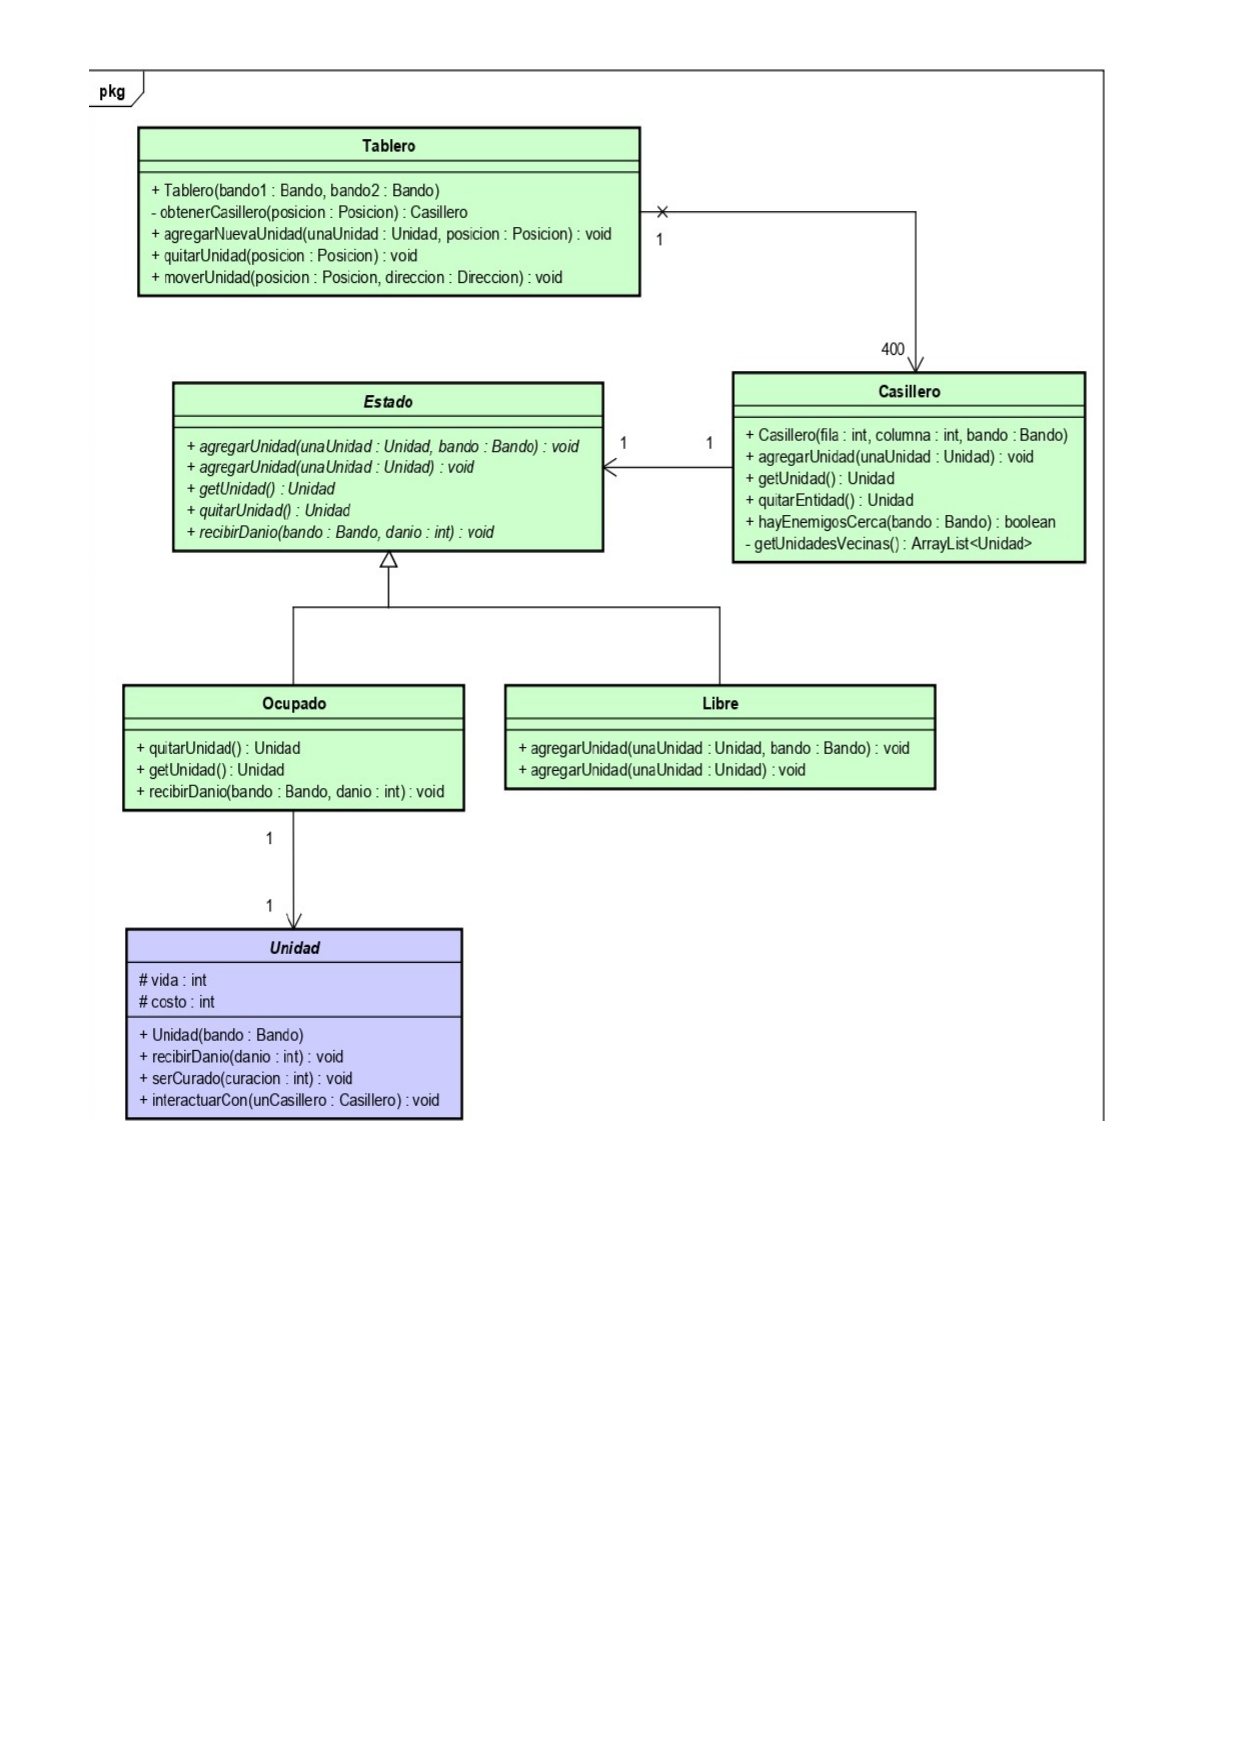
\includegraphics[width=0.8\textwidth]{TABLEROV1_page-0001.jpg}
\caption{\label{fig:class01}Diagrama del Tablero.}

\end{figure}


\begin{figure}[H]
\centering
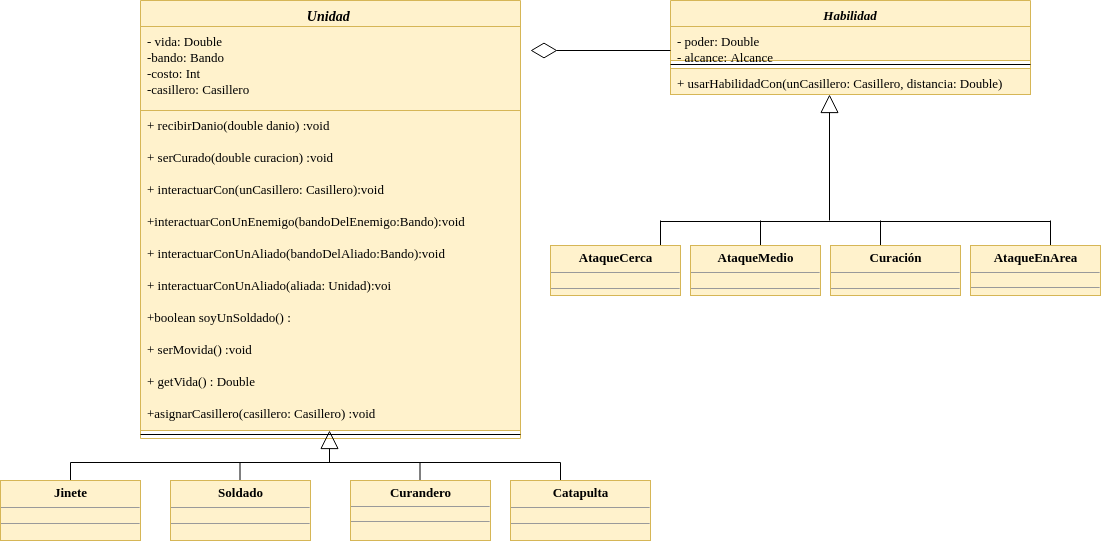
\includegraphics[width=0.8\textwidth]{DiagramaClaseUnidad.png}
\caption{\label{fig:class01}Diagrama de Clase Unidad.}
\end{figure}


\begin{figure}[H]
\centering
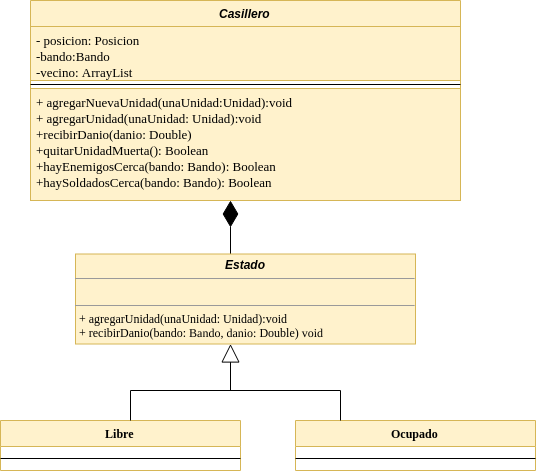
\includegraphics[width=0.8\textwidth]{DDiagEstado.png}
\caption{\label{fig:class01}Diagrama de Clase Casillero detallado.}
\end{figure}



\section{Detalles de implementación}\label{sec:implementacion}
% Explicaciones sobre la implementación interna de algunas clases que consideren que puedan llegar a resultar interesantes.

Nos resulta interesante entrar en detalles de implementación de los siguientes temas: 


\subsection{Movimiento}

Moverse de una posición a otra:  

La clase Posición se encarga de definir la posición nueva que se corresponde con un determinado movimiento efectuado en una dirección. Para realizar el movimiento, una posición (instanciada) recibirá un argumento del tipo Dirección que corresponde a la dirección en la que debe moverse. 
La dirección pasada por argumento es la que se usará para informarle a la posición el método al que debe invocar según la dirección que se indique en cada caso. 

\begin{verbatim}

\end{verbatim}

\subsection{Ataque}
Atacar en Área:  

Para lograr un ataque en área se trabaja paralelamente guardando los casilleros de las unidades que no fueron atacadas y con los de las ya atacadas. En principio, el ataque corresponderá a la unidad que se busca dañar, ésta será guardada como no atacada, luego de atacarla, dejará de estar guardada como unidad sin atacar y pasará a formar parte de las que se guardan como atacadas. Pero los casilleros vecinos de la unidad que acaba de ser dañada, se guardarán como no atacados, para atacarlos y así pasar a formar parte de la lista de casilleros ya atacados. Esto será un ciclo que finalizará cuando no haya casilleros no atacados guardados o se encuentre que el casillero contiguo a una unidad atacada está vacío y por lo tanto el ataque en área finaliza según las reglas establecidas del juego. 

\subsection{State Pattern}

El estado de un casillero:

Un casillero está asociado a un Estado. Libre y ocupado son las subclases de la superclase Estado. Un casillero siempre se encuentra en alguno de esos dos estados y puede pasar de uno a otro en el transcurso del juego.
Por ejemplo, al comenzar el juego, todos los casilleros se encuentran libres pero cuando un jugador coloca una unidad en alguno éste pasa de libre a ocupado. Para esta implementación se utilizó el patrón de diseño 'State Pattern' la principal razón de uso fue para encapsular el comportamiento variable para el mismo objeto, en función de su estado interno. 

\subsection{Herencia}

Herencia: 

Durante el diseño del trabajo se decidió usar herencia en varias oportunidades: La unidad, la habilidad y la dirección. En todos los casos fue utilizada con motivo y justificación de reutilización de toda la interfaz. 



\section{Excepciones}\label{sec:excepciones}
% Explicación de cada una de las excepciones creadas y con qué fin fueron creadas.

\begin{description}
\item[CasilleroLibreException] Sus fines de creación fueron atrapar las siguientes acciones inválidas:  \\ \hspace{}
- Se busca quitar una unidad de un casillero libre.  \\ \hspace{}
-Se busca obtener unidades vecinas de un casillero vacío, hecho que carece de sentido en la lógica planteada del juego. \\ \hspace{}
-En el caso de la búsqueda de formación de un batallón, la excepción surge como validación. Es decir, si en alguno de los sentidos (horizontal, vertical, etc) en los que se busca un batallón hay un casillero libre, entonces allí no hay un batallón. \\ \hspace{}
- Si se intenta atacar un casillero vacío al realizar un ataque en área. 
\item[CasilleroOcupadoExcepcion] Sus fines de creación fueron atrapar las siguientes acciones inválidas: \\ \hspace{}
- Se busca agregar una unidad a un casillero ocupado. \\ \hspace{}
-Se intenta mover a algún integrante de un batallón a un casillero ocupado.
\item[CatapultaNoPuedeSerCuradaExcepcion] Se intenta curar una catapulta cuando, según las reglas del juego, eso no es posible. 
\item[DesplazamientoInvalidoExcepcion] Sus fines de creación fueron atrapar las siguientes acciones inválidas:\\ \hspace{}
- Se intenta realizar un desplazamiento fuera del rango posible. 
\item[DistanciaInvalidaExcepcion] Si la distancia entre dos casilleros supera o es inferior a los rangos de distancia máxima y mínima respectivamente. 
\item[DistintoBandoExcepcion] Se utiliza para detectar si la unidad está interactuando con un enemigo. 
\item[MismaUnidadExcepcion] Se utiliza para detectar si la unidad está interactuando con ella misma. 
\item[MismoBandoExcepcion] Se utiliza para detectar si la unidad está interactuando con una de su mismo bando. 
\item[PosicionInvalidaExcepcion] Se utiliza para detectar si una posición es invalida. \\ \hspace{}
\item[PuntosInsuficientesExcepcion] El jugador intenta agregar una unidad sin los puntos suficientes para hacerlo. 
\\ \hspace{}
\end{description}

\section{Diagramas de secuencia}\label{sec:diagramasdesecuencia}
% Mostrar las secuencias interesantes que hayan implementado. Pueden agregar texto para explicar si algo no queda claro.


\begin{figure}[H]
\centering
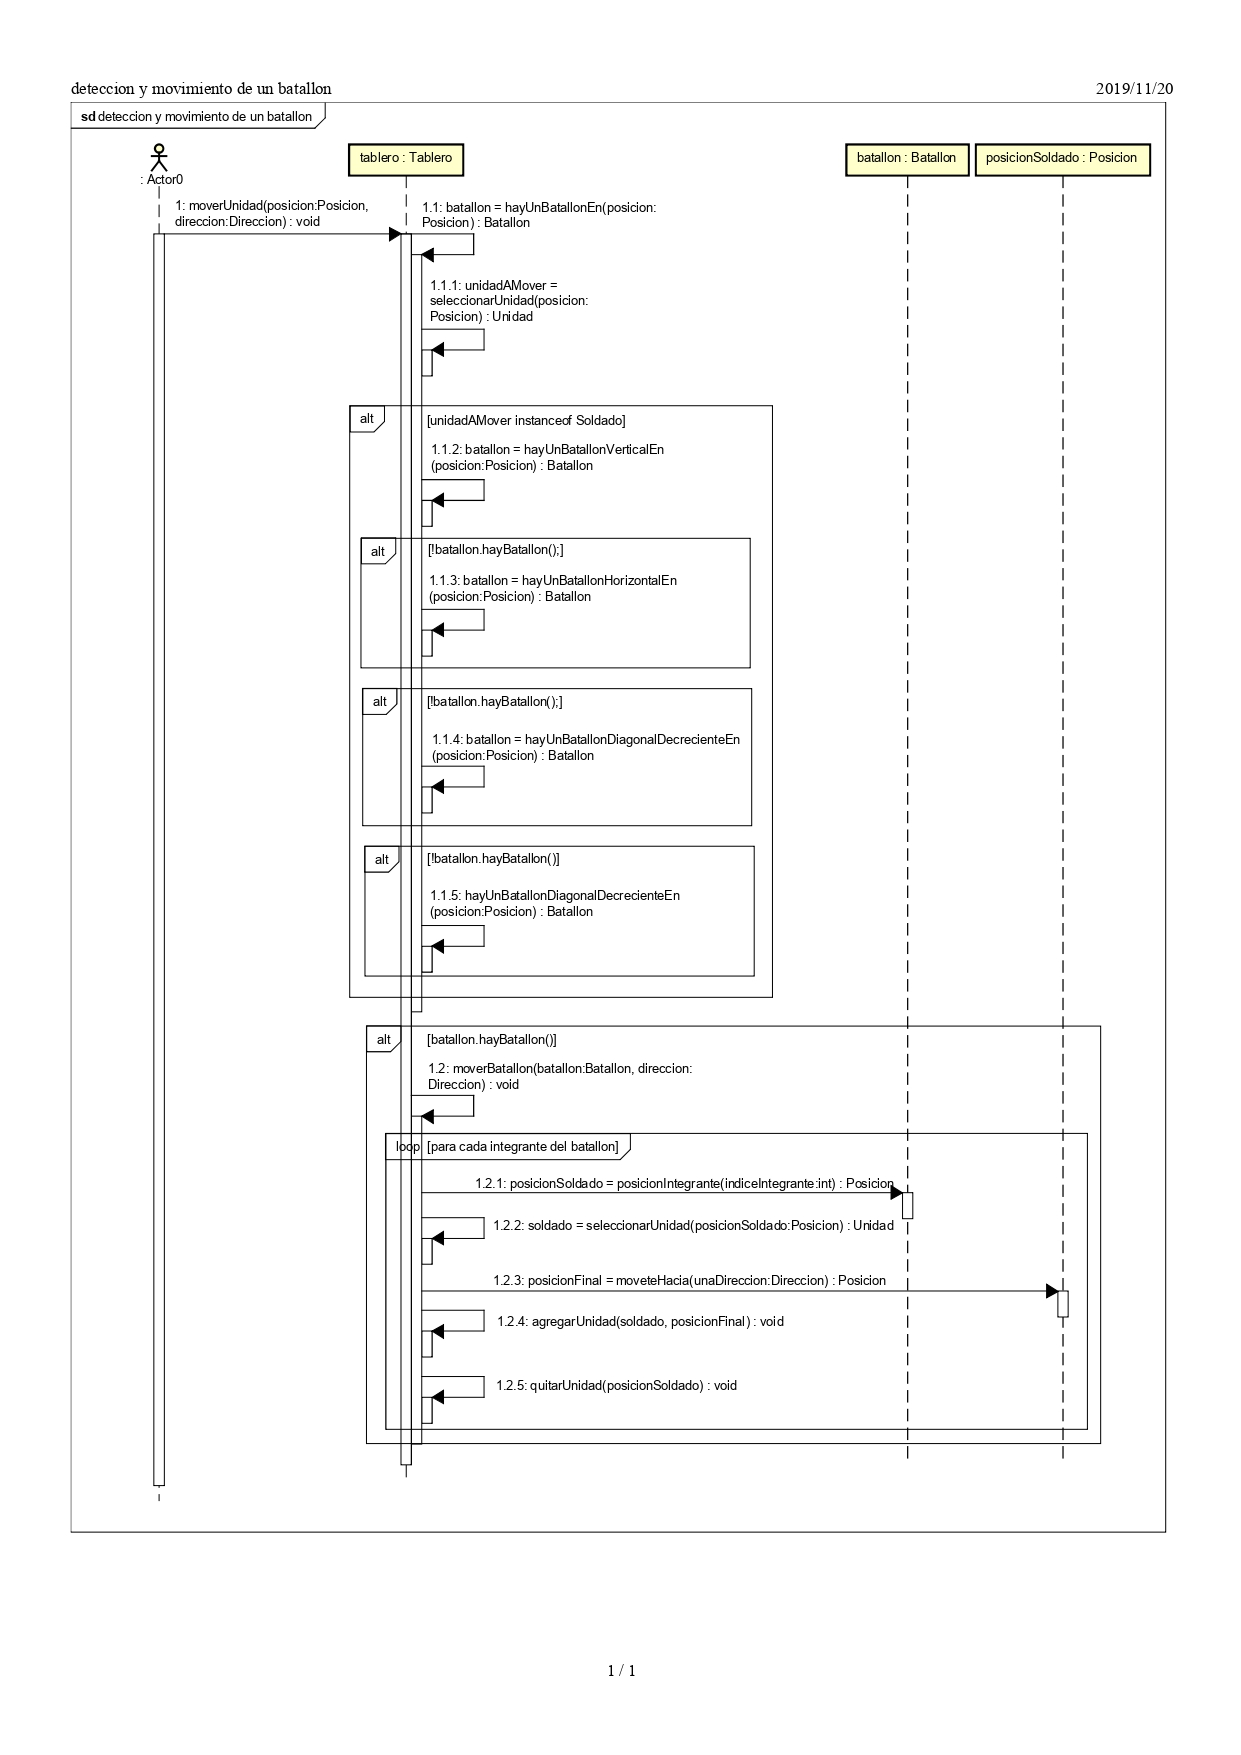
\includegraphics[width=0.8\textwidth]{1- Deteccion y movimiento de un batallon.jpg}
\caption{\label{fig:seq01}. Detección y movimiento de un Batallón}
\end{figure}


\begin{figure}[H]
\centering
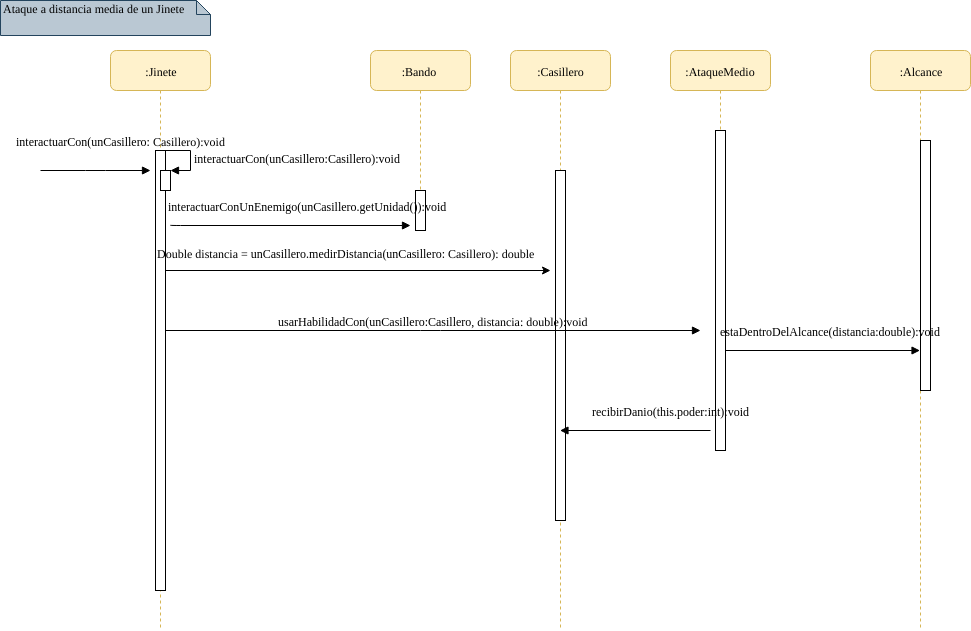
\includegraphics[width=\textwidth]{AtaqueJinete.png}
\caption{\label{fig:seq02}Ataque de un Jinete a distancia media}
\end{figure}

\begin{figure}[H]
\centering
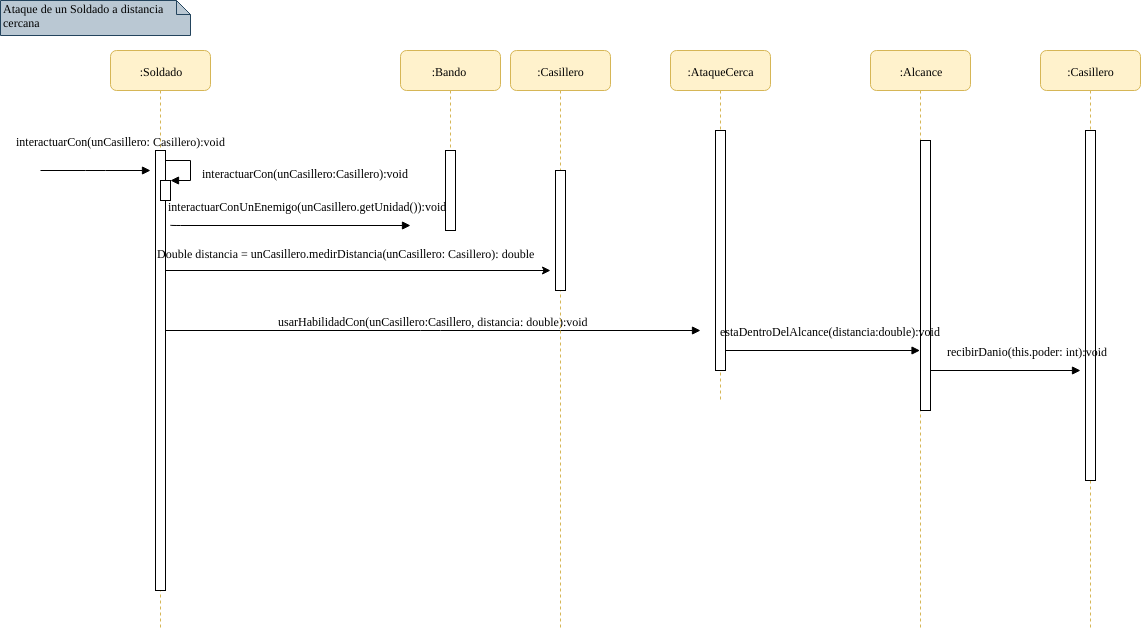
\includegraphics[width=\textwidth]{AtaqueSoldado.png}
\caption{\label{fig:seq02}Ataque a distancia cercana de un Soldado}
\end{figure}


\begin{figure}[H]
\centering
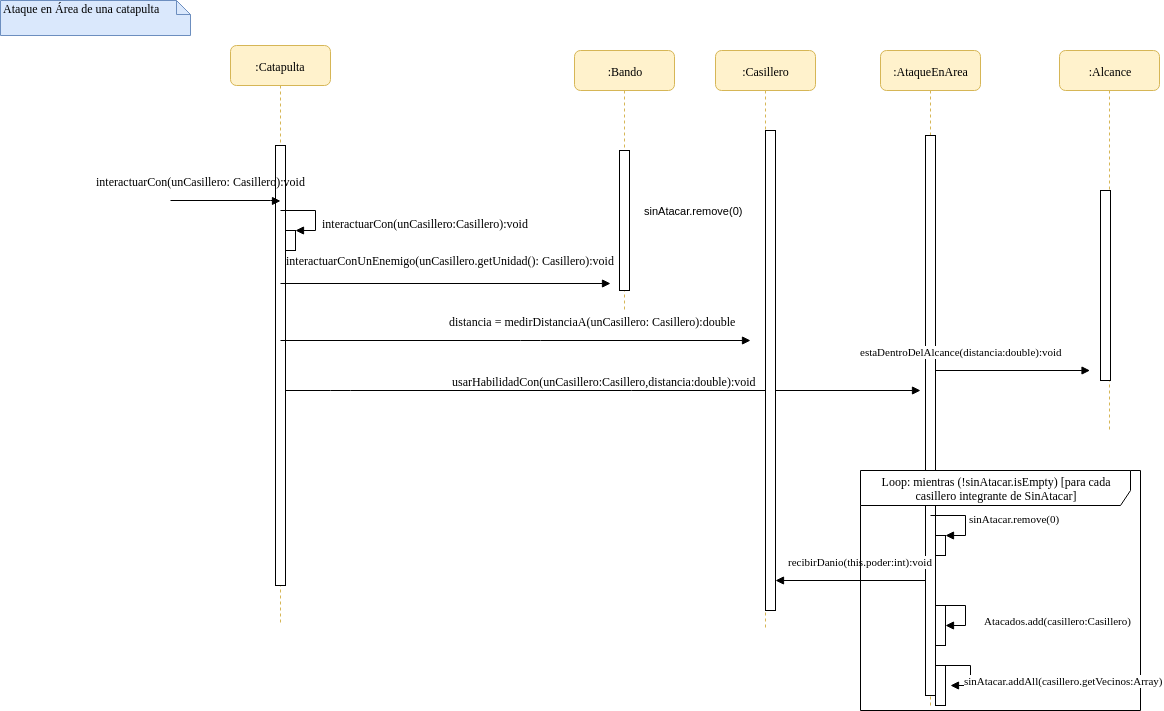
\includegraphics[width=\textwidth]{AtaqueCatapulta.png}
\caption{\label{fig:seq02}Ataque en área de una catapulta}
\end{figure}

\begin{figure}[H]
\centering
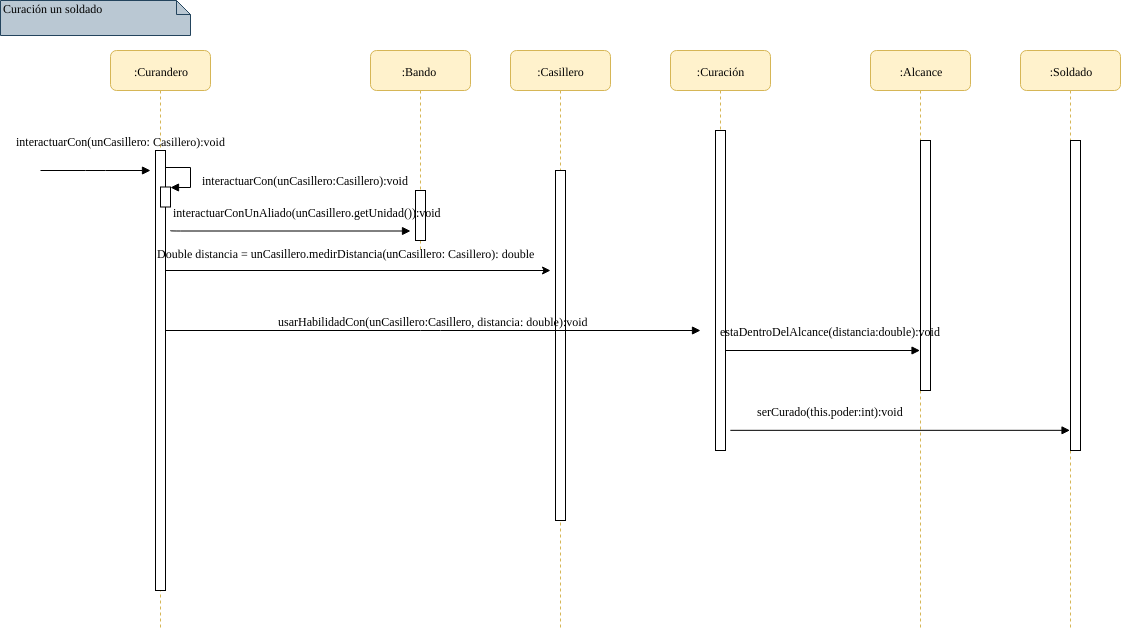
\includegraphics[width=\textwidth]{Curacion (1).png}
\caption{\label{fig:seq02}Curación de un Soldado. Se deja como ejemplo concreto de secuencia de curación la de un soldado, pero la secuencia sería idéntica para cualquier unidad que no sea una Catapulta, ya que ésta no puede ser curada.}
\end{figure}




\section{Diagramas de estado}\label{sec:diagramasdesecuencia}
% Mostrar las secuencias interesantes que hayan implementado. Pueden agregar texto para explicar si algo no queda claro.


\begin{figure}[H]
\centering
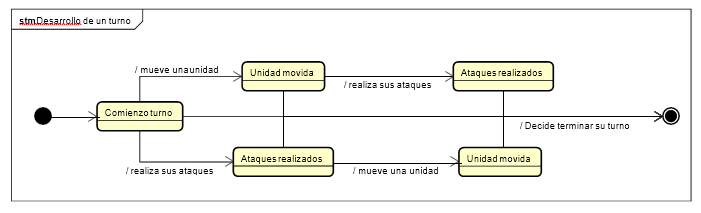
\includegraphics[width=0.8\textwidth]{Turno.png}
\caption{\label{fig:seq01}. Turno}
\end{figure}




\end{document}
